\newpage
\section{NOTA TEÓRICA}

Antes de iniciar con el desarrollo del presente proyecto, es necesario tener a mano una serie de conceptos importantes, los cuales se explican a continuación: 

\subsection{Placa NODEMCU ESP8266 WIFI}

La placa NodeMCU ESP8266 es una plataforma de desarrollo muy accesible y de bajo costo, basada en el microcontrolador ESP8266. Este microcontrolador de 32 bits utiliza la arquitectura Tensilica Xtensa LX106 y puede operar a una frecuencia de entre 80 MHz y 160 MHz. Una de sus características más destacadas es su capacidad Wi-Fi integrada, lo que permite que la placa se conecte a redes Wi-Fi y funcione tanto como punto de acceso como cliente, lo que la hace ideal para proyectos de Internet de las Cosas (IoT).

La NodeMCU ESP8266 ofrece 17 pines GPIO (General Purpose Input/Output) para conectar sensores, actuadores y otros periféricos (4 pueden configurarse como PWM a 3.3V). También incluye pines para comunicación I2C, SPI, UART, ADC, entre otros. Su programación es muy accesible, ya que puede hacerse usando el entorno de desarrollo Arduino IDE, lo que la hace ideal para principiantes y entusiastas. Además, puede programarse en lenguaje Lua a través del firmware NodeMCU.

El microcontrolador ESP8266 cuenta con una memoria flash interna, de 4 MB, que permite almacenar el firmware y otros datos necesarios para el funcionamiento del dispositivo. Gracias a sus capacidades Wi-Fi y su bajo costo, la NodeMCU ESP8266 es utilizada en una amplia variedad de proyectos, desde la automatización del hogar hasta sistemas de monitoreo remoto y dispositivos IoT.

La placa puede ser alimentada mediante un cable micro-USB o a través de los pines de alimentación (VIN y GND), con un voltaje de funcionamiento de 3.3V. Además, es compatible con plataformas de desarrollo como Blynk, facilitando la creación de aplicaciones móviles para controlar y monitorear dispositivos conectados.

A continuación se puede ver el Diagrama de pines de la placa:

\begin{figure}[H]
\centering
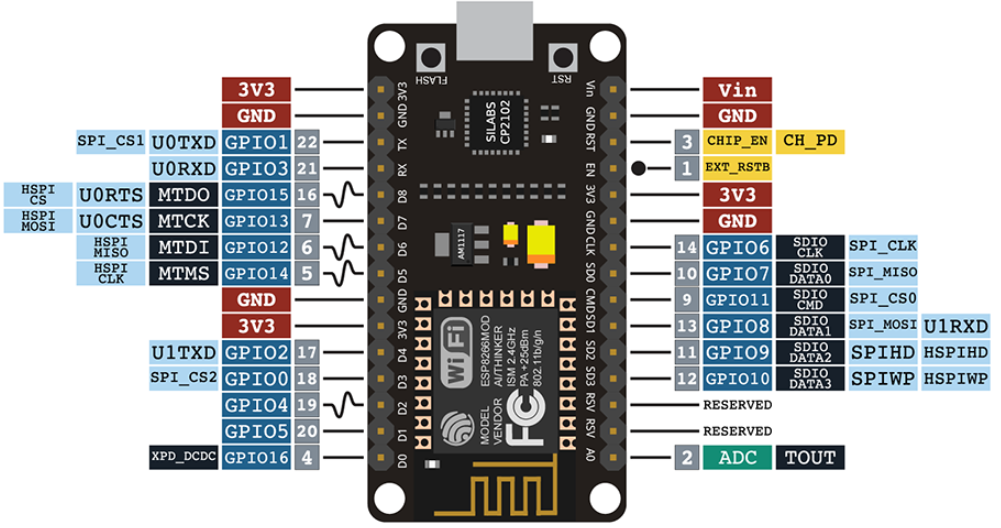
\includegraphics[width=120mm]{./Figuras/Nota_teorica/PINOUT_PLACA}
\caption{Diagrama de Pines NodeMCU ESP8266. (Fuente: \cite{Acrobotic_2016})}
\label{fig:HC}
\end{figure}

\subsubsection{Características Eléctricas: ESP8266}
A continuación se muestran las caracteristicas electricas del ESP8266 según su hoja del fabricante \cite{EspressifSystems_2023}:

\begin{table}[H]
    \centering
    \scriptsize
    \begin{tabular}{|l|l|c|c|c|c|}
        \hline
        \textbf{Parameters} & \textbf{Conditions} & \textbf{Min} & \textbf{Typical} & \textbf{Max} & \textbf{Unit} \\ \hline
        Operating Temperature Range & - & -40 & Normal & 125 & C \\ \hline
        Maximum Soldering Temperature & IPC/JEDEC J-STD-020 & - & - & 260 & C \\ \hline
        Working Voltage Value & - & 2.5 & 3.3 & 3.6 & V \\ \hline
        $V_{IL}$ & - & -0.3 & - & 0.25 $V_{IO}$ & V \\ \hline
        $V_{IH}$ & - & 0.75 $V_{IO}$ & - & 3.6 & V \\ \hline
        $V_{OL}$ & - & - & - & 0.1 $V_{IO}$ & V \\ \hline
        $V_{OH}$ & - & 0.8 $V_{IO}$ & - & - & V \\ \hline
        $I_{max}$ & - & - & - & 12 & mA \\ \hline
        Electrostatic Discharge (HBM) & TAMB = 25  C & - & - & 2 & KV \\ \hline
        Electrostatic Discharge (CDM) & TAMB = 25  C & - & - & 0.5 & KV \\ \hline
    \end{tabular}
    \caption{Características eléctricas NodeMCU ESP8266}
    \label{table:nodemcu_parameters}
\end{table}
\subsubsection{Diagrama de bloques: ESP8266}
A continuación se muestra el Diagrama de bloques del ESP8266 según su hoja del fabricante \cite{EspressifSystems_2023}:

\begin{figure}[H]
\centering
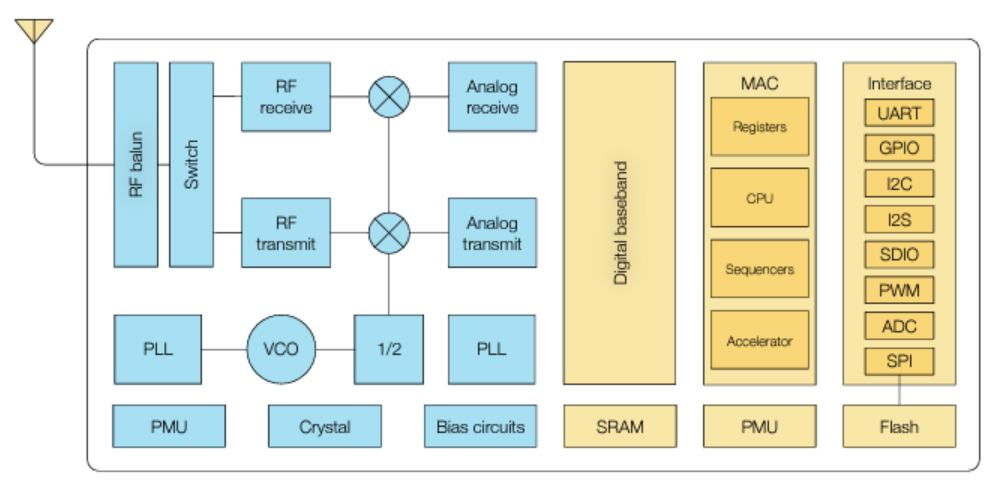
\includegraphics[width=120mm]{./Figuras/Nota_teorica/Diagrama_de_bloques_micro}
\caption{Diagrama de bloques ESP8266. (Fuente: \cite{EspressifSystems_2023})}
\label{fig:esp1}
\end{figure}

\subsection{Librerías de importancia}
A continuación se detallan las librerías que fueron utilizadas en el proyecto:

\begin{itemize}
    \item \underline{\texttt{ESP8266WiFi.h}}: permite al ESP8266 conectarse a redes WiFi. Proporciona funciones para escanear redes disponibles, conectar o desconectar de una red, y obtener información sobre la conexión actual, como la intensidad de la señal y la dirección IP asignada.
    
    \item \underline{\texttt{BlynkSimpleEsp8266.h}}: diseñada para integrar el ESP8266 con la plataforma Blynk. Permite conectar el dispositivo a la aplicación móvil Blynk para crear interfaces de usuario con botones, \textit{sliders} y otros \textit{widgets} para controlar el ESP8266 y recibir datos en tiempo real.

    \item \underline{\texttt{Servo.h}}: permite controlar servomecanismos con el ESP8266. Proporciona funciones para configurar el ángulo del servo motor, establecer la velocidad de movimiento, y otras operaciones básicas necesarias para controlar servos en proyectos de robótica o automatización.
\end{itemize}

\subsection{IoT: Internet of things}
El Internet de las cosas (IoT, por sus siglas en inglés) se refiere a una red abierta y completa de objetos inteligentes que tienen la capacidad de autoorganizarse, compartir información, datos y recursos, reaccionando y actuando ante situaciones y cambios en el entorno. Es un concepto que ha evolucionado desde la idea de que la primera versión de Internet trataba sobre datos creados por personas, mientras que la siguiente versión se trata de datos creados por cosas \cite{madakam2015internet}. 

\subsection{Sensores ultrasónicos (HC-SR04)}
El HC-SR04 es un sensor de distancia ultrasónico que se destaca por su bajo costo y facilidad de uso. Este sensor es capaz de medir distancias en un rango de 2 cm a 400 cm, lo que lo convierte en una herramienta popular en proyectos de robótica y automatización para evitar obstáculos y medir distancias \cite{HC}. A continuación se detallan los pasos del funcionamiento del sensor: 

\begin{enumerate}
    \item \textbf{Emisión de onda ultrasónica}: el sensor está equipado con dos transductores ultrasónicos: uno para enviar las ondas (transmisor) y otro para recibirlas (receptor). Cuando se activa el pin Trig (\textit{Trigger}) enviando un pulso alto de al menos 10 µs, el sensor emite una serie de ondas ultrasónicas a una frecuencia de 40 kHz.

    \item \textbf{Reflexión de onda}: las ondas ultrasónicas viajan a través del aire y se reflejan en un objeto situado frente al sensor.

    \item \textbf{Recepción de onda}: el transductor receptor detecta las ondas reflejadas y genera un pulso en el pin Echo. La duración de este pulso es proporcional al tiempo que tardaron las ondas en viajar al objeto y regresar al sensor.

    \item \textbf{Cálculo de distancia}: La distancia se calcula utilizando la siguiente fórmula: 

    \begin{equation*}
        Distancia (d) = \frac{V \times T}{2}
    \end{equation*}

    Donde $V$ es es la velocidad del sonido en el aire y $T$ es el tiempo medido en microsegundos ($\mu$s) desde el envío hasta la recepción de las ondas.
\end{enumerate}

En la Figura \ref{fig:HC}, puede consultarse el comportamiento descrito, además de la disposición de pines: 

\begin{figure}[H]
\centering
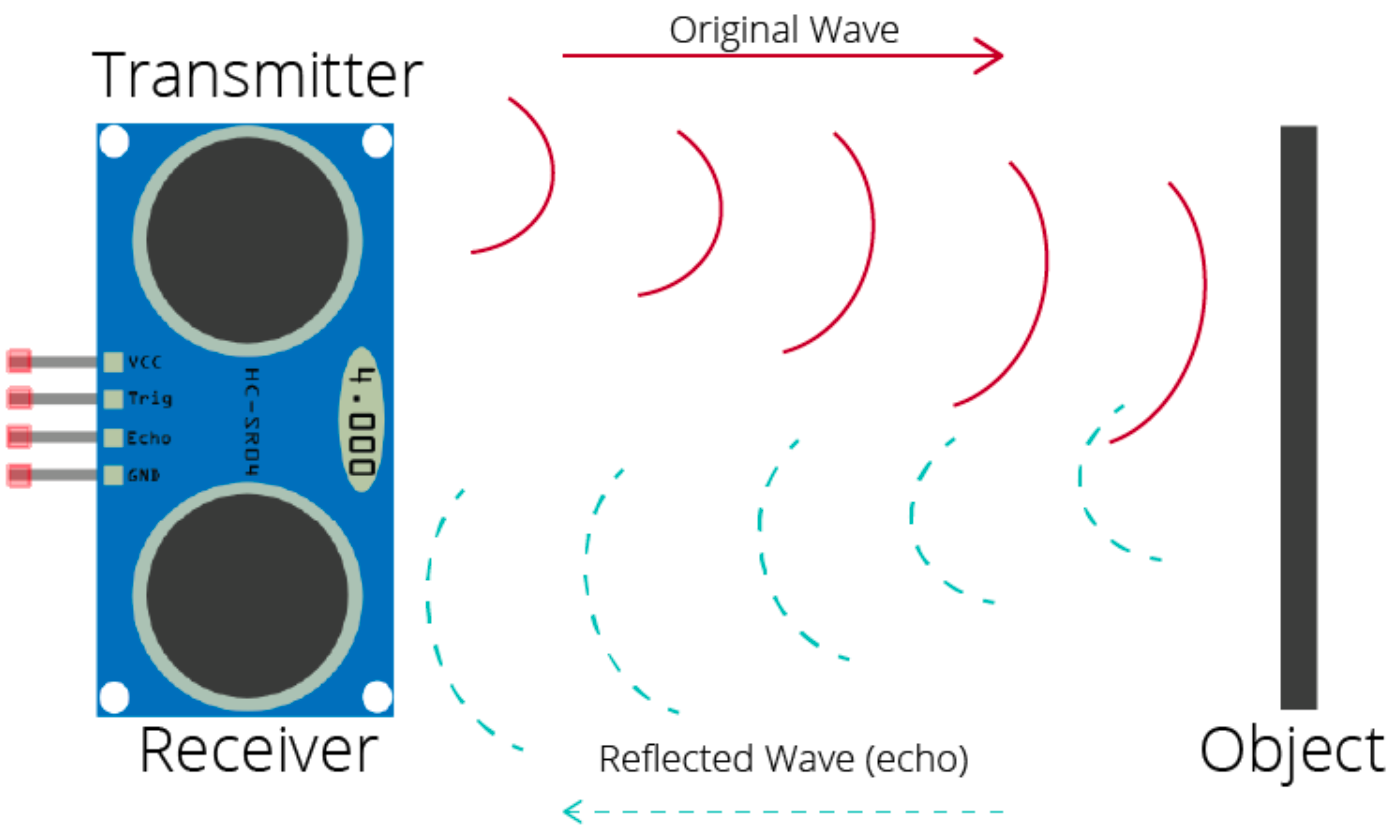
\includegraphics[width=120mm]{./Figuras/Nota_teorica/HC}
\caption{Funcionamiento del sensor ultrasónico HC-SR04 y disposición de pines del dispositivo. (Fuente: \cite{RNT})}
\label{fig:HC}
\end{figure}

\subsection{Servo motor del kit de Arduino}
Según se detalla en \cite{SM}, un servomotor es un dispositivo de actuador utilizado en diversos campos como la robótica, vehículos RC y modelos aéreos. Se destaca por su capacidad de control preciso de posición, lo que lo hace adecuado para tareas que requieren movimientos exactos y de alta fuerza. 

Un servomotor típico está compuesto por un motor eléctrico, un potenciómetro, electrónica de control y una caja de engranajes. El potenciómetro mide la posición actual del eje, y la electrónica de control compara esta posición con la posición deseada, ajustando el motor para mantener la posición del eje en el valor objetivo. Este proceso de ajuste continuo constituye un sistema de control en bucle cerrado. Lo anterior puede apreciarse de manera gráfica en la Figura \ref{fig:SM}: 

\begin{figure}[H]
\centering

\includegraphics[width=120mm]{./Figuras/Nota_teorica/SM}
\caption{Composición de un servo motor. (Fuente: \cite{SM})}
\label{fig:SM}
\end{figure}

Para conectar un servomotor a un microcontrolador, se deben conectar tres cables: alimentación (VCC) a 5V, tierra (GND) a GND, y señal a un pin digital del dispositivo de control. Es fundamental considerar que, si se utilizan múltiples servos o servos de mayor tamaño, se debe utilizar una fuente de alimentación externa para evitar dañar el microcontrolador.

\subsection{Bomba de agua}
Tal como se describe en \cite{BA}, este componente cuenta con un motor de 6V y 0.25A de alta resistencia, un cuerpo de plástico termoplástico resistente, y es completamente sumergible, aunque también puede funcionar en seco sin dañarse. La bomba, opera a un rango de voltaje de 2.5 a 6V, ofrece una elevación máxima de 40 a 110 cm y un caudal de 80 a 120 L/h. Sus dimensiones son un diámetro de aproximadamente 24 mm, una longitud de 45 mm y una altura de 33 mm. Equipado con un motor magnético sin escobillas y una vida útil de 500 horas de funcionamiento continuo, este dispositivo es ideal para aplicaciones diversas como fuentes, cascadas, y sistemas de riego automatizados, garantizando un movimiento eficiente y confiable del agua. En la Figura \ref{fig:WP}, puede observarse el tipo de mini bomba de agua que se utilizará en el proyecto: 

\begin{figure}[H]
\centering
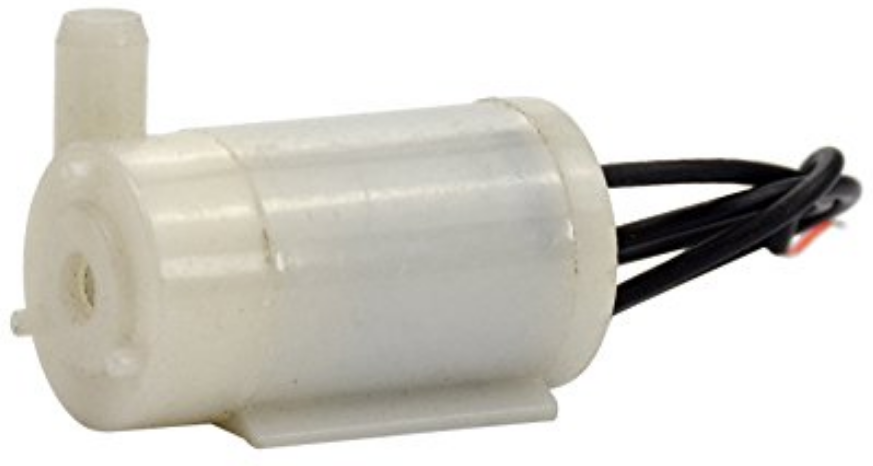
\includegraphics[width=100mm]{./Figuras/Nota_teorica/WP}
\caption{Mini-bomba de agua. (Fuente: \cite{BA})}
\label{fig:WP}
\end{figure}

Una bomba de agua funciona mediante un impulsor que gira para crear una fuerza centrífuga, lo que genera una baja presión en el centro y succiona el agua hacia el interior de la bomba a través del puerto de succión. El agua es entonces empujada hacia afuera mediante la presión generada y dirigida a través del puerto de descarga gracias al diseño de la voluta. El motor impulsa el impulsor, y en algunos casos, la bomba necesita ser primada para eliminar el aire y asegurar un flujo continuo de agua \cite{ST}.

\subsection{Blynk IoT}

Tal como se explica en \cite{BK}, Blynk es una plataforma en la nube para IoT de bajo código que simplifica la creación, implementación y gestión de aplicaciones IoT. Permite construir aplicaciones móviles y web personalizables sin necesidad de programación, gestionar dispositivos, datos y actualizaciones, y garantizar seguridad empresarial en todo el ciclo de vida del IoT. Blynk puede ser conectado con varios dispositivos como SP32, ESP8266, Arduino Uno, Raspberry Pi, Particle Photon, Seeed Wio Terminal y TI CC3220 y ofrece diversos métodos para conectar dispositivos a su plataforma en la nube:

\begin{itemize}
    \item \textbf{Blynk Library}: Una biblioteca C++ que proporciona una conexión bidireccional de baja latencia entre el dispositivo y la nube de Blynk, manteniendo el dispositivo siempre conectado.

    \item \textbf{Blynk.Edgent}: Una solución empaquetada que incluye Blynk.Inject para provisión dinámica de credenciales y Blynk.Air para actualizaciones de firmware OTA, ideal para hardware compatible con esta opción.

    \item \textbf{Blynk.NCP}: Una pila de software para módulos de procesamiento de red (NCP) que maneja la conectividad (WiFi, Ethernet, Celular), permitiendo al MCU principal usar una biblioteca cliente ligera para la comunicación.

    \item \textbf{HTTP(s) API}: Un protocolo estándar que permite a los dispositivos conectarse periódicamente a la nube para transferir datos, ideal para dispositivos celulares que envían datos en lotes.

    \item \textbf{MQTT API}: Un protocolo de comunicación bidireccional seguro que admite autenticación, actualizaciones de datos, eventos y más, ideal para proyectos que utilizan bibliotecas MQTT o plataformas similares.
\end{itemize}

Estos métodos ofrecen flexibilidad en el desarrollo y gestión de aplicaciones IoT, adaptándose a diferentes necesidades y tipos de hardware \cite{BK}.

\subsection{Lista de componentes y precios}
En la Tabla \ref{table:Equipo} pueden consultarse los componentes utilizados y sus precios tomando como referencia los precios del sitio web de la tienda de componentes MicroJPM (\url{https://www.microjpm.com/}): 

\begin{table}[H]
\caption{Lista de componentes.}
\begin{center}
\begin{tabular}{c|c|c}
\hline
\textbf{Componente}&\textbf{Cantidad}&\textbf{Precio}\\
\hline
NodeMCU ESP8266 & 1 & \$10,95\\
Batería de 9 V & 1 & \$5.64\\
Servo motor & 1 & \$5,95\\
Mini bomba agua sumergible & 1 & \$5,50\\
Resistor de  2 k$\Omega$ & 2 & \$0,80\\
Transistor 2N2222 & 1 & \$0,25\\ 
Relé & 1 & \$1.08\\
Diodo & 1 & \$0.095\\ 
Jumpers & 60 & \$6.90\\
Materiales de construcción & - & \$11.71\\
Mano de obra & - & \$19.99\\
\hline
Total & - & \$68.86\\
\end{tabular} \label{table:Equipo}
\end{center}
\end{table}

% Poner el precio en colones

Según la Tabla \ref{table:Equipo}, para realizar este proyecto son necesarios ₡36176.15, según el valor del dólar al momento de escribir el presente informe. 